\documentclass[journal]{IEEEtran}
\usepackage[T1]{fontenc}
\usepackage{amsmath,amssymb,graphicx,array,cite,capt-of,float}
\usepackage{url,xcolor}
\newcommand{\bluecite}[1]{\textcolor{blue}{\cite{#1}}}
\begin{document}
\setcounter{section}{0}
\section{Introduction}
Encrypted-traffic classification supports network management and security monitoring. As encryption becomes widespread, traffic analysis increasingly relies on observable packet bytes, lengths, directions, and timing to identify applications, services, and attacks. Pretrained models, hierarchical representations, and graph neural networks learn these signals from complementary perspectives~\cite{ch2-1,ch2-2,ch2-3,ch2-4,ch2-5,ch2-6,ch2-7,ch2-8}. In operational networks, however, applications and attacks evolve, and classes absent from training may appear at test time. A classifier restricted to predefined labels can assign such traffic to a known class. Encrypted-traffic recognition must therefore classify known traffic while rejecting unseen classes.

Existing unknown-traffic detectors use discriminative or generative criteria. Classifier confidence and feature boundaries can separate known from unknown traffic, but unknown samples may receive high confidence. FEC-OSL~\cite{ch2-10} learns an energy boundary with auxiliary unknown traffic; this requirement limits its use when only known-class samples are available. Open-Detect~\cite{ch2-15} uses generative and discriminative constraints to learn Gaussian class prototypes and rejects samples according to their prototype distances. A prototype summarizes the class globally. When within-class support is uneven, a point near the prototype can still lie far from the observed training samples. Local sample neighborhoods can therefore complement global class position.

We propose TriGLE (Tri-view Global-Local Empirical support framework) for open-set encrypted-traffic recognition. Byte sequences, packet interactions, and multilevel byte organization form a fused representation. Empirical class centroids and within-class nearest neighbors measure a test flow's deviation from known traffic. We calibrate the rejection threshold using only known-class validation data, without auxiliary unknown training flows.

Our contributions are as follows:
\begin{enumerate}
\item We combine byte context, packet interactions, and multilevel byte organization through Gaussian adaptation and deterministic fusion to represent encrypted flows for classification and rejection.
\item We integrate empirical centroid distance with within-class neighbor distance and calibrate normalization and rejection using known-class validation data.
\item We evaluate known-class recognition, unknown-service and attack rejection, and component contributions on ISCX-VPN, ISCX-Tor, USTC-TFC2016, CIC-IDS2017, and VNAT. In the four VNAT complete-service holdout folds, the method attains mean AUROC of 99.22\% and UFAR of 1.09\%. On identical representations, local support raises mean AUROC from 97.43\% with centroids alone to 99.22\%.
\end{enumerate}

Section~II reviews related work, Section~III describes the method, Section~IV reports the experiments, and Section~V concludes the paper.

\section{Related Work}
\subsection{Encrypted-Traffic Classification}
Encrypted-traffic classifiers learn representations that distinguish traffic classes using observable packet attributes such as bytes, lengths, directions, and timing. Sequence models capture byte context and relationships across packets. ET-BERT~\cite{ch2-1} pretrains contextualized datagram representations on large volumes of unlabeled traffic and fine-tunes them for downstream classification. TrafficFormer~\cite{ch2-2} combines fine-grained multiclass pretraining with packet-field augmentation to improve traffic representations. MIETT~\cite{ch2-3} treats each flow as a set of packet instances and models both within-packet and cross-packet relationships through two-level attention, packet position prediction, and flow-level contrastive learning.

Hierarchical and graph-based approaches capture additional aspects of traffic structure. YaTC~\cite{ch2-4} arranges packet headers and payloads in multilevel matrices and combines packet-level and flow-level attention with masked pretraining to preserve byte organization and cross-packet structure. GraphDApp~\cite{ch2-5} models bidirectional communications as flow interaction graphs and identifies decentralized applications with a graph neural network. TFE-GNN~\cite{ch2-6} uses pointwise mutual information to build byte association graphs, encodes headers and payloads separately, and combines them through cross-gated fusion. MH-Net~\cite{ch2-7} uses multigranular heterogeneous graphs to model headers, payloads, and their relationships jointly. DigTraffic~\cite{ch2-8} constructs message-aware flow interaction graphs and uses a dual-channel graph Transformer to fuse length and timing features. These approaches capture complementary aspects of hierarchical organization, communication interactions, and byte associations.

Most of these classifiers target predefined classes and do not explicitly reject unknown classes~\cite{ch2-1,ch2-2,ch2-3,ch2-4,ch2-6,ch2-7}. Accurate discrimination among known classes does not ensure reliable detection of unknown traffic. GraphDApp and DigTraffic both include open-world evaluations. GraphDApp includes unmonitored traffic in training~\cite{ch2-5}, while DigTraffic primarily evaluates binary discrimination between seen and unseen traffic~\cite{ch2-8}. Maintaining fine-grained classification while reliably rejecting unknown classes using only known-class training data remains an open problem.

\subsection{Unknown-Traffic Detection Methods}
Unknown-traffic detection aims to classify known traffic accurately and reject traffic from classes absent during training. The main approaches use discriminative or generative modeling, with some methods also supporting class discovery and incremental updates.

\subsubsection{Discriminative Unknown-Traffic Detection}
Discriminative methods separate known and unknown traffic using classifier outputs, partitions of feature space, or feature distances. Zhang et al.~\cite{ch2-9} use classification confidence to screen candidate unknown samples and update the classifier through a self-learning discriminator, clustering, and automatic labeling. FEC-OSL~\cite{ch2-10} combines dual-branch feature extraction with energy boundary learning to distinguish known and unknown traffic. It uses auxiliary unknown data and deep clustering to separate unknown traffic into finer categories. FOSS~\cite{ch2-11} uses isolation trees to partition feature space, detect local anomalies, and distinguish unknown attacks. It adapts to changes in legitimate traffic through incremental updates. RFG-HELAD~\cite{ch2-12} combines latent features from contrastive learning and a generative adversarial network. It uses nearest-neighbor distances in the learned feature space to detect unknown attacks and a heterogeneous ensemble to improve robustness. These methods extend detection criteria beyond classification confidence to spatial structure and sample neighborhoods. Their requirements for auxiliary data and model updates differ.

\subsubsection{Generative Unknown-Traffic Detection}
Generative methods use reconstruction or probability distributions to model known classes and detect test samples that deviate from those patterns. Trident~\cite{ch2-13} uses multiple autoencoder-based one-class learners and class-specific anomaly thresholds to reject unknown samples. Clustering supports new-class discovery and incremental updates. Yang et al.~\cite{ch2-14} combine a conditional variational autoencoder with extreme value theory to identify unknown attacks from reconstruction errors and their tail distributions. They also cluster benign traffic to reduce false alarms. Open-Detect~\cite{ch2-15} uses Gaussian class prototypes with generative and discriminative constraints to improve within-class compactness and between-class separation. It rejects unknown samples according to their distances from the prototypes. Reconstruction and distribution modeling provide complementary criteria for unknown-traffic detection. Class prototypes capture global structure, while nearest-neighbor measures capture support from local training samples. Combining these signals under known-class-only training remains an open direction.

\subsection{Summary}
Prior studies have improved encrypted-traffic classification and unknown-traffic detection through different representations and decision criteria. One open direction is to fuse byte sequences, packet interactions, and multilevel byte structure while combining global class distributions with local neighborhood information to support known-class classification and unknown-class rejection.

\section{Method}
TriGLE combines representation learning with global and local empirical support for open-set encrypted-traffic recognition. The method characterizes traffic through byte sequences, packet interactions, and multilevel byte organization, and constructs a unified representation through Gaussian adaptation and deterministic fusion. It then combines empirical class centroids with within-class sample neighborhoods to measure deviations from known classes in terms of both global position and local neighborhood relationships. The resulting rejection score integrates global and local information for known-class classification and unknown-class rejection. Fig.~3-1 presents the overall framework.
\begin{figure*}[!t]
\centering
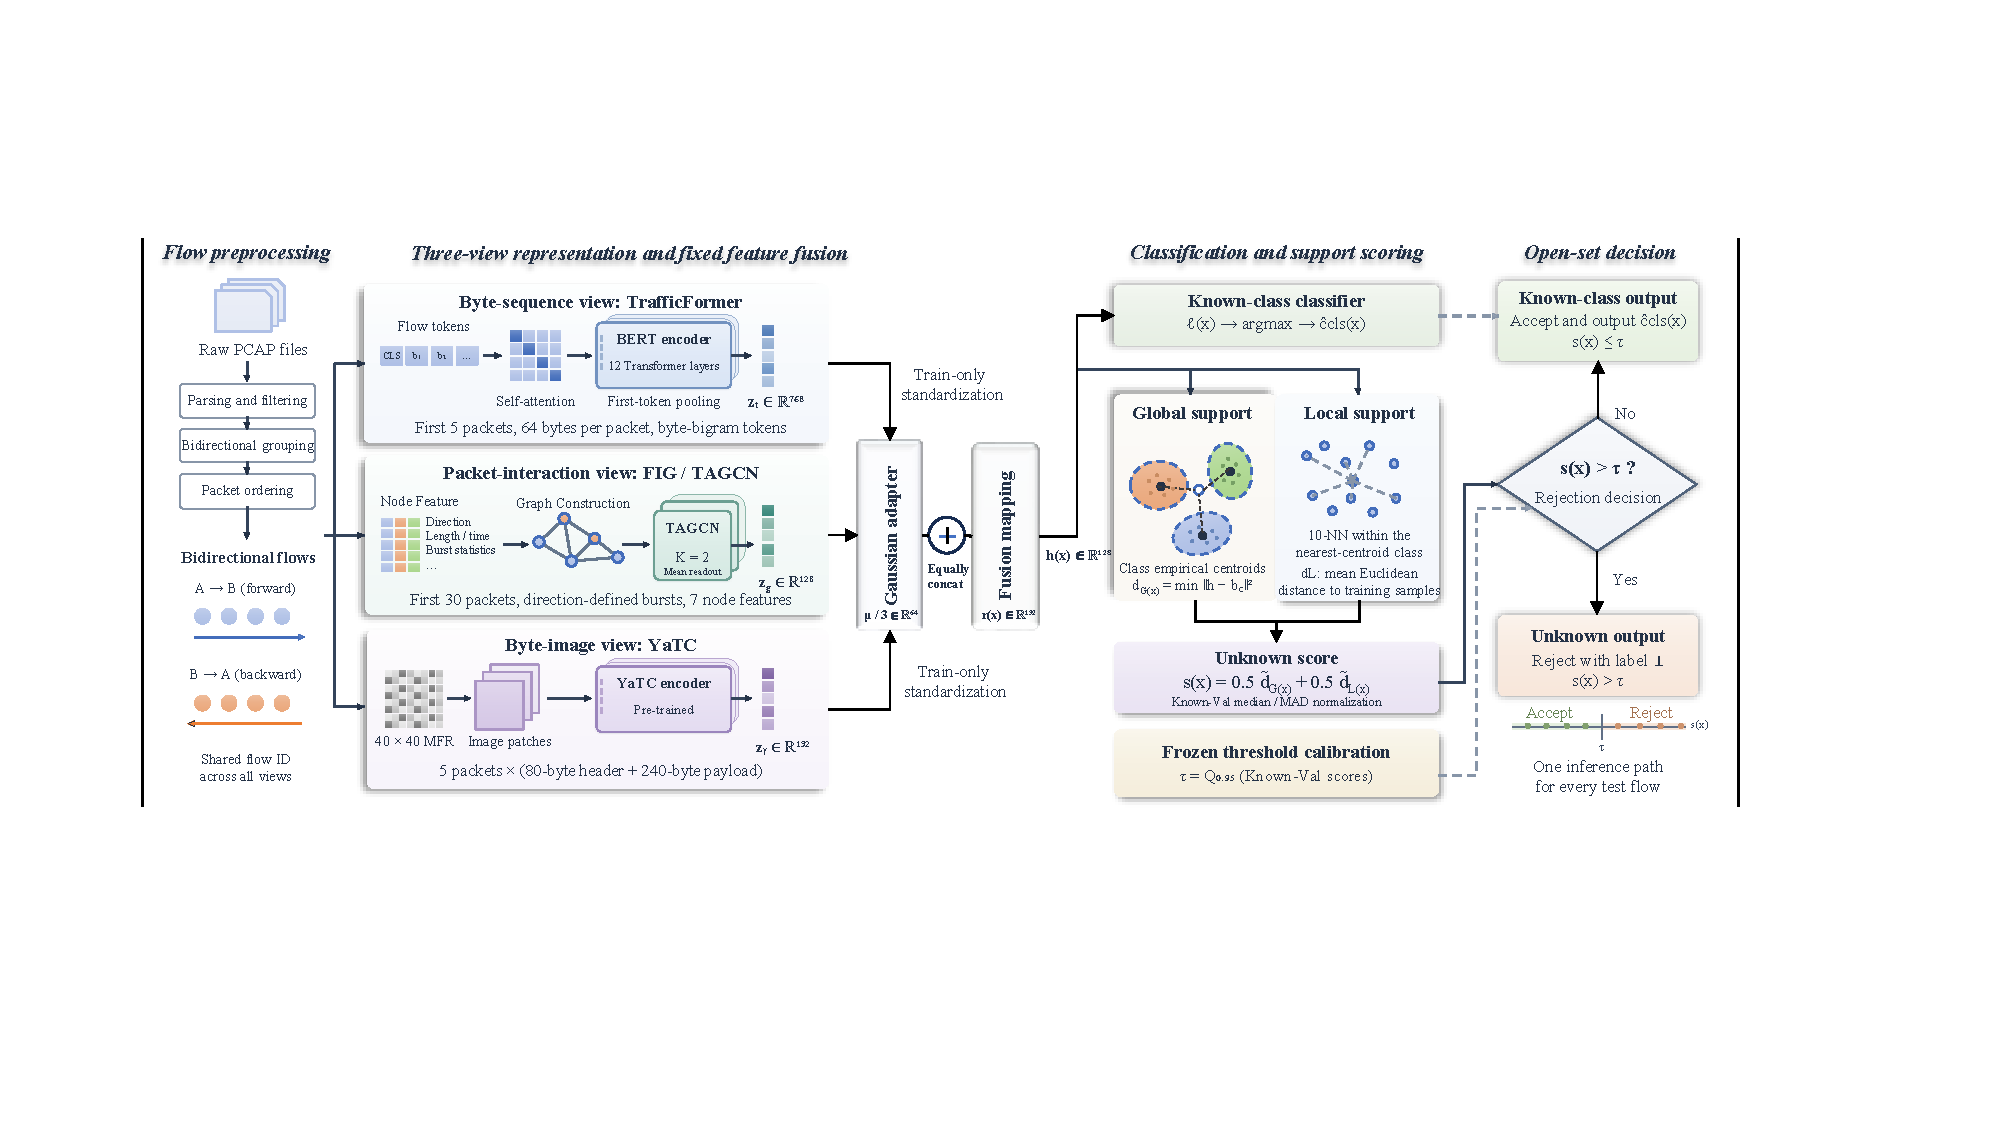
\includegraphics[width=\textwidth,trim=61bp 141bp 119bp 108bp,clip,keepaspectratio]{images/suggestion3_framework.pdf}
\begingroup\renewcommand{\thefigure}{3-1}
\caption{Overall framework of the proposed method.}
\label{fig:framework}\endgroup
\end{figure*}

\subsection{Problem Definition and Notation}
In open-set encrypted-traffic recognition, the labeled training set contains $N$ samples, $\mathcal{D}_{\mathrm{tr}}=\{(x_i,y_i)\}_{i=1}^{N}$. Here, $x_i\in\mathcal{X}$ denotes a bidirectional flow, $\mathcal{X}$ is the traffic sample space, and $y_i\in\mathcal{C}_K=\{1,\ldots,C\}$ is its class label, with $C$ known classes. The known-class validation set is $\mathcal{D}_{\mathrm{val}}$, whose labels also belong to $\mathcal{C}_K$.

At test time, the model processes traffic from both the known-class set $\mathcal{C}_K$ and the unknown-class set $\mathcal{C}_U$. Unknown classes appear in neither the training set nor the validation set, and $\mathcal{C}_K\cap\mathcal{C}_U=\varnothing$. Test samples therefore extend beyond the classes observed during training.

Our objective is to learn an open-set recognition model $f$ that maps an input flow to a known-class label or a unified unknown label:
\begin{equation}
f:\mathcal{X}\rightarrow\mathcal{C}_K\cup\{\bot\},
\tag{1}
\end{equation}
Here, $\bot$ denotes the unknown label. The learning objective has two parts: (1) accurately distinguish flows in $\mathcal{C}_K$ and output their known-class labels; and (2) identify flows in $\mathcal{C}_U$ and assign them the unified unknown label. The model thus addresses both known-class classification and unknown-class rejection. Table~3-1 summarizes the main notation; other symbols are defined at first use.

\begin{table}[!t]\centering\begingroup
\renewcommand{\thetable}{3-1}
\caption{Main notation and definitions}\label{tab:notation}
\fontsize{8}{9.5}\selectfont\setlength{\tabcolsep}{3pt}
\begin{tabular}{@{}p{.31\columnwidth}p{.64\columnwidth}@{}}\hline
Symbol & Definition \\\hline
$\mathcal C_K,\mathcal C_U$ & Known- and unknown-class sets \\
$\mathcal D_{\mathrm{tr}},\mathcal D_{\mathrm{val}}$ & Known training and validation sets \\
$z_v(x),\mu_v(x)$ & Encoded view features and latent mean after Gaussian adaptation \\
$h(x),\ell(x)$ & Fused features and known-class classification score vector \\
$\mathcal T_c,b_c$ & Training representation set and empirical centroid of class $c$ \\
$c^*(x)$ & Class of the nearest centroid \\
$d_G(x),d_L(x)$ & Global centroid distance and local nearest-neighbor distance \\
$s(x),\tau$ & Combined rejection score and rejection threshold \\\hline
\end{tabular}\endgroup\end{table}

\subsection{Traffic Representation Learning in TriGLE}
Encrypted-traffic class characteristics appear in byte combinations and contextual relationships, interactions between packets, and the internal hierarchical structure of packets. We construct byte-sequence, flow-interaction-graph, and byte-image views to learn byte-context dependencies, packet interactions, and multilevel byte organization, respectively. Let $x=\{p_1,p_2,\ldots,p_{n_x}\}$ denote the chronologically ordered packet sequence of a bidirectional flow, where $n_x$ is the packet count. The sending direction of the first packet defines the forward direction. Each branch constructs its input from the same flow and extracts complementary flow-level features for subsequent Gaussian adaptation and fusion.

\subsubsection{Byte-Sequence Branch}
The byte-sequence branch captures local byte-combination patterns and contextual dependencies along the packet-byte sequence. We use pretrained TrafficFormer~\cite{ch2-2} as the byte-sequence encoder to map raw packet bytes to a flow-level sequence representation.

For the chronologically ordered flow $x=\{p_1,p_2,\ldots,p_{n_x}\}$, we select the first $\min(5,n_x)$ packets. After removing the Ethernet header, we retain at most 64 bytes per packet and form hexadecimal byte bigrams following the TrafficFormer input representation. For a byte sequence $(b_1,b_2,\ldots,b_m)$, the bigram representation is $(b_1\Vert b_2,b_2\Vert b_3,\ldots,b_{m-1}\Vert b_m)$, where $\Vert$ denotes concatenation of adjacent bytes. TrafficFormer's token mapping converts these combinations into discrete tokens, which form a flow-level sequence in the original packet order. After adding the $[\mathrm{CLS}]$ token, we truncate or pad the input to a maximum of 320 tokens.

Let $T(x)$ denote the resulting token sequence. We extract features using the pretrained TrafficFormer encoder and fine-tune it with supervision on the known-class training set. The hidden representation at the $[\mathrm{CLS}]$ position in the final encoder layer serves as the flow-level byte-sequence feature:
\begin{equation}
z_t(x)=E_{\mathrm{TF}}\!\left(T(x)\right)_{\mathrm{CLS}}
\in\mathbb{R}^{768},
\tag{2}
\end{equation}
Here, $E_{\mathrm{TF}}$ is the fine-tuned TrafficFormer encoder, and $z_t(x)$ is the 768-dimensional byte-sequence representation used by the subsequent multiview adaptation and fusion module.

\subsubsection{Flow-Interaction-Graph Branch}
The flow-interaction-graph branch characterizes communication behavior through relationships between packets, complementing the low-level content features of the byte-sequence branch. Following existing Flow Interaction Graph (FIG) modeling approaches~\cite{ch2-10,ch2-5}, we represent a bidirectional flow as a packet-level graph. A Topology Adaptive Graph Convolutional Network (TAGCN) learns a structured interaction representation that captures transmission direction, timing, and interaction topology.

For the chronologically ordered flow $x=\{p_1,p_2,\ldots,p_{n_x}\}$, we construct a graph from the first $\min(30,n_x)$ packets, with one node per packet. Consecutive packets with the same sending direction form a burst. Within each burst, edges connect consecutive packets in temporal order. Between adjacent bursts, edges connect their first nodes and their last nodes, capturing transmission continuity and direction changes. This procedure produces an undirected flow interaction graph $G(x)=(V,E)$, where $V$ and $E$ denote the node and edge sets. Fig.~3-2 illustrates burst segmentation, graph construction, node features, and neighborhood aggregation.

\begin{figure}[H]\centering
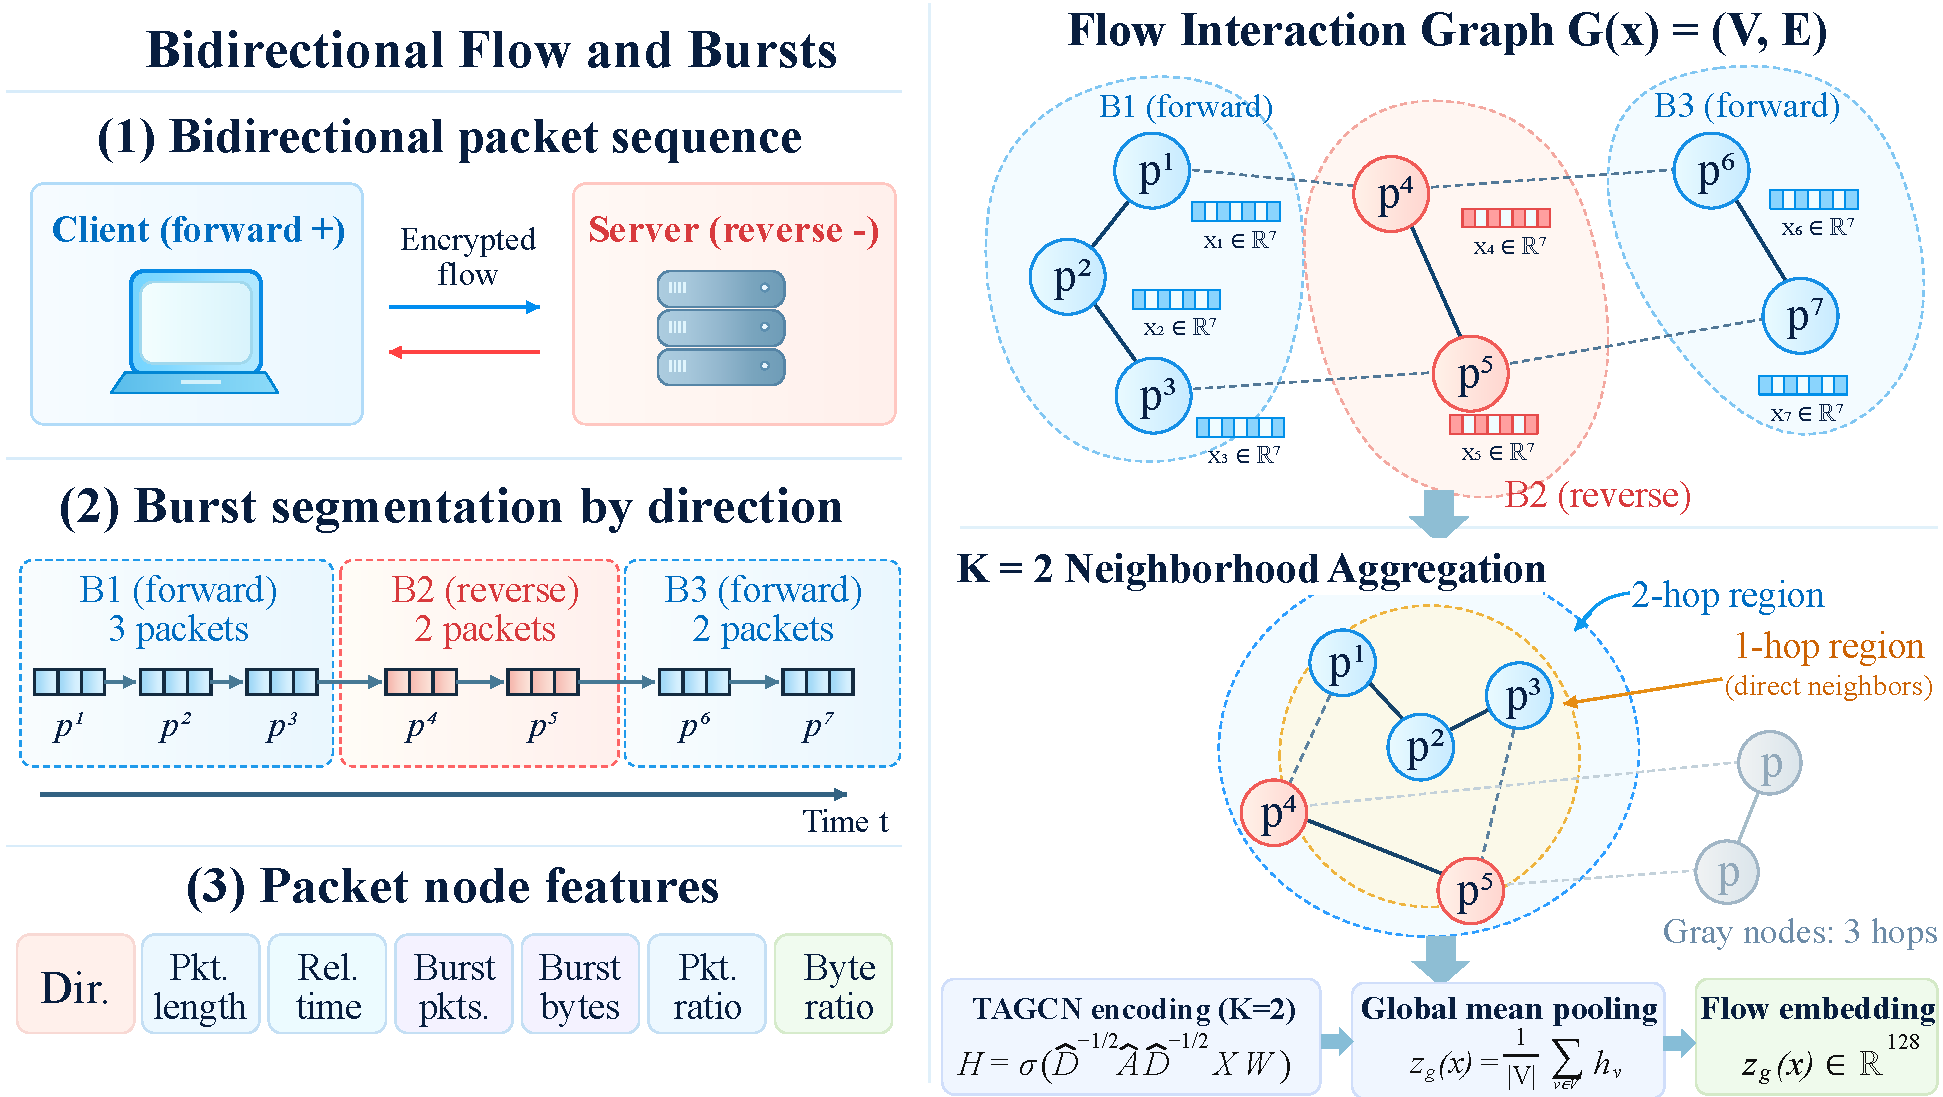
\includegraphics[width=\columnwidth,keepaspectratio]{images/flow-interaction-graph.pdf}
\begingroup\renewcommand{\thefigure}{3-2}
\caption{Flow interaction graph construction and neighborhood aggregation.}
\label{fig:flow-graph}\endgroup\end{figure}

Each node has seven interaction features: sending direction, packet length, elapsed time relative to the first packet, the packet count and total byte count of its burst, and the ratios of the current burst's packet and byte counts to those of the preceding burst. These features describe transmission attributes, local interaction scale, and changes between transmission stages. We collect packet nodes from flows in the known-class training set and compute the mean and standard deviation of each feature dimension. Dimension-wise standardization yields the node-feature matrix $X\in\mathbb{R}^{|V|\times7}$. Validation and testing reuse the training statistics.

TAGCN aggregates neighborhoods of multiple orders to learn structural dependencies between packets. Let $A$ denote the adjacency matrix, with normalized form $\hat{A}=D^{-1/2}(A+I)D^{-1/2}$, where $D$ is the degree matrix of $A+I$. The node-feature update is
\begin{equation}
H=\operatorname{ReLU}\left(
\sum_{k=0}^{2}\hat{A}^{k}XW_k+b
\right),
\tag{3}
\end{equation}
Here, $W_k$ and $b$ are learnable parameters, and $H\in\mathbb{R}^{|V|\times128}$ combines node attributes and multihop topology. Global mean pooling then produces the flow-level graph feature:
\begin{equation}
z_g(x)=\frac{1}{|V|}\sum_{u\in V}H[u,:]
\in\mathbb{R}^{128},
\tag{4}
\end{equation}
The resulting 128-dimensional representation $z_g(x)$ serves as input to multiview adaptation and fusion.

\subsubsection{Byte-Image Branch}
Packet headers and payloads exhibit hierarchical byte organization beyond byte-sequence patterns and packet interactions. Direct concatenation of raw bytes can allocate excessive representation space to longer packets and discard structural information from other packets. Following YaTC's Multi-Level Flow Representation (MFR)~\cite{ch2-4}, we organize raw bytes into a two-dimensional matrix with a fixed layout. Hierarchical encoding captures byte-, packet-, and flow-level structure.

For a bidirectional flow $x$, we select the first five packets and retain an 80-byte header region and a 240-byte payload region per packet, padding missing content with zeros. The fixed header and payload positions form an $8\times40$ packet-level matrix. Stacking these matrices in chronological order yields the $40\times40$ flow-level MFR matrix:
\begin{equation}
B(x)=\operatorname{Stack}(M_1,M_2,\ldots,M_5)
\in\mathbb{R}^{40\times40},
\tag{5}
\end{equation}
Here, $M_i$ is the two-dimensional byte matrix of packet $i$, containing separate header and payload regions. Fixed spatial positions for bytes at different levels preserve within-packet structure and flow-level organization. We normalize byte values to $[-1,1]$ before encoding.

The pretrained YaTC encoder partitions the MFR matrix into nonoverlapping patches and constructs initial features through linear projection and positional embeddings. Packet-level attention first extracts byte relationships within packets, and row pooling (RP) aggregates them into row-level representations:
\begin{equation}
U_p=E_{\mathrm{PL}}(B(x)),\qquad
U_r=\operatorname{RP}(U_p),
\tag{6}
\end{equation}
Here, $E_{\mathrm{PL}}$ comprises patch embedding and packet-level attention, $U_p$ is the packet-level representation, and $U_r$ is the representation after row pooling.

Flow-level attention then models dependencies across packets, and column pooling (CP) produces the flow-level representation:
\begin{equation}
U_f=E_{\mathrm{FL}}(U_r),\qquad
z_y(x)=\operatorname{CP}(U_f)\in\mathbb{R}^{192},
\tag{7}
\end{equation}
Here, $E_{\mathrm{FL}}$ is the flow-level attention encoder, $U_f$ is its output, and $z_y(x)$ is the final 192-dimensional byte-image feature. We initialize the encoder with pretrained YaTC parameters and fine-tune it with supervision on the known-class training set. The resulting multilevel byte features feed the adaptation and fusion module.

\subsection{Gaussian Adaptation and Deterministic Feature Fusion}
The three views capture byte context, packet interactions, and multilevel byte organization, but their feature dimensions and numerical scales differ. We first standardize each encoded view feature $z_v(x)$ using known-training-set statistics, then map it into a common latent space with a view-specific Gaussian adapter. Let $v\in\{t,g,y\}$ index the byte-sequence, flow-interaction-graph, and byte-image views, respectively. The conditional distribution of each latent representation is
\begin{equation}
q_v(u\mid x)
=
\mathcal{N}
\left(
\mu_v(x),
\operatorname{diag}\left(\exp(a_v(x))\right)
\right),
\tag{8}
\end{equation}
Here, $\mu_v(x)$ and $a_v(x)$ denote the latent mean and log variance, respectively. All views share latent dimension $d_u$.

Gaussian adaptation jointly optimizes class discrimination and latent-distribution constraints. During training, reparameterized sampling from $q_v(u\mid x)$ produces latent representations. Classification cross-entropy preserves information relevant to known classes, while KL divergence from the standard normal distribution regularizes the latent distribution. The adaptation objective is
\begin{equation}
\begin{aligned}
\mathcal{L}_{\mathrm{adapt}}={}&\frac{1}{3M}\sum_{i=1}^{M}\sum_{v\in\{t,g,y\}}\Bigl[\mathcal L^{\mathrm{CE}}_{iv}\\
&+\frac{\beta}{d_u}D_{\mathrm{KL}}\left(q_v(u\mid x_i)\,\|\,\mathcal N(0,I)\right)\Bigr].
\end{aligned}\tag{9}
\end{equation}
Here, $M$ is the batch size. For sample $i$ and view $v$, $\mathcal L^{\mathrm{CE}}_{iv}$ is the classification cross-entropy between the true label and the prediction of a view-specific classifier operating on the reparameterized latent sample. The coefficient $\beta$ controls distribution regularization. The classification term preserves class differences, while the KL term constrains deviations from the standard normal distribution.

To eliminate randomness from latent sampling in distance calculations, we construct a deterministic fused representation from the latent means. We scale all three means by the same coefficient, concatenate them, and apply a learnable mapping to obtain fused features. A classification head outputs known-class scores:
\begin{equation}
\begin{aligned}
r(x)&=
\operatorname{concat}
\left(
\frac{\mu_t(x)}{3},
\frac{\mu_g(x)}{3},
\frac{\mu_y(x)}{3}
\right),\\
h(x)&=F_{\varphi}(r(x))\in\mathbb{R}^{128},\\
\ell(x)&=g_{\psi}(h(x))\in\mathbb{R}^{C}.
\end{aligned}
\tag{10}
\end{equation}
Here, $r(x)$ is the concatenated representation, $F_{\varphi}$ learns combinations of features across views, and $g_{\psi}$ is the known-class classification head. The score $\ell_c(x)$ corresponds to class $c$. Global and local empirical support modeling also uses $h(x)$, placing known-class classification and unknown-class discrimination in the same representation space.

\subsection{Global and Local Empirical Support Modeling}
Known-class classification distinguishes classes, whereas unknown-class discrimination must also assess a test sample's relationship to known training samples. Class centroids summarize the overall location of training representations but cannot fully characterize within-class distributions. A sample near a centroid may still lie far from actual training samples. We therefore combine class centroids and within-class nearest neighbors in the fused space to characterize deviations in global position and local proximity. In the learned, fixed representation space, known training samples define a reference set for each class:
\begin{equation*}
\begin{gathered}
\mathcal{T}_c=\{h(x_i):y_i=c,(x_i,y_i)\in\mathcal{D}_{\mathrm{tr}}\},
\\
N_c=|\mathcal{T}_c|.
\end{gathered}
\end{equation*}
Here, $\mathcal T_c$ is the training representation set of known class $c$, and $N_c$ is its size. The mean representation $b_c$ serves as the empirical centroid, summarizing the class's overall position. For a test flow $x$, distances to all class centroids determine the nearest-centroid class $c^*(x)$. The corresponding squared Euclidean distance defines the global distance $d_G(x)$:
\begin{equation}
\begin{aligned}
b_c&=\frac{1}{N_c}\sum_{h_i\in\mathcal{T}_c}h_i,\\
c^*(x)&=\operatorname*{arg\,min}_{c\in\mathcal{C}_K}
\|h(x)-b_c\|_2^2,\\
d_G(x)&=\|h(x)-b_{c^*(x)}\|_2^2.
\end{aligned}
\tag{11}
\end{equation}
The global distance measures deviation from the nearest class centroid. To characterize proximity to actual training representations, we select the $k$ representations nearest to $h(x)$ in Euclidean distance from $\mathcal{T}_{c^*(x)}$. These representations form the local neighborhood $\mathcal{N}_k(x)$. The local distance is their mean distance to the test representation:
\begin{equation}
d_L(x)=
\frac{1}{k}
\sum_{h_j\in\mathcal{N}_k(x)}
\|h(x)-h_j\|_2,
\qquad
\mathcal{N}_k(x)\subseteq\mathcal{T}_{c^*(x)}.
\tag{12}
\end{equation}
A larger $d_L(x)$ indicates greater separation from the selected class's training neighborhood and thus weaker local empirical support. Global and local distances provide complementary geometric evidence of deviation from the class's overall location and actual training neighborhood. The nearest-centroid class $c^*(x)$ selects the class for neighborhood construction. The classification head still determines the final known-class label of an accepted sample; the two class assignments need not agree.

\subsection{Robust Standardization and Open-Set Decision}
The global distance $d_G(x)$ is a squared Euclidean distance to a centroid, whereas $d_L(x)$ is a mean Euclidean distance to within-class neighbors. Their numerical scales differ, so direct combination can allow one distance to dominate. We robustly standardize them separately using the known-class validation set. For $a\in\{G,L\}$, let $\mathcal{S}_a=\{d_a(x):x\in\mathcal{D}_{\mathrm{val}}\}$. Its median $m_a$ and median absolute deviation $\mathrm{MAD}_a$ describe location and dispersion, yielding
\begin{equation}
\begin{gathered}
m_a=\operatorname{median}(\mathcal{S}_a),\\
\mathrm{MAD}_a=\operatorname{median}_{u\in\mathcal{S}_a}|u-m_a|,
\\
\tilde d_a(x)=\frac{d_a(x)-m_a}{\mathrm{MAD}_a+\varepsilon}.
\end{gathered}\tag{13}
\end{equation}
Here, the positive constant $\varepsilon>0$ prevents division by zero. Fixed equal weights combine the standardized distances into the rejection score $s(x)$. The empirical 95\% quantile of known-validation scores determines the threshold $\tau$:
\begin{equation}
\begin{gathered}
s(x)=\frac{1}{2}\tilde d_G(x)+\frac{1}{2}\tilde d_L(x),
\\
\tau=Q_{0.95}\left(\{s(x):x\in\mathcal{D}_{\mathrm{val}}\}\right).
\end{gathered}\tag{14}
\end{equation}
Here, $Q_{0.95}$ denotes the empirical quantile operator. Both the standardization statistics and the rejection threshold come from the known-class validation set. A higher $s(x)$ indicates greater combined deviation from known-class centroids and training neighborhoods. Scores above the threshold trigger an unknown decision. Otherwise, the classification head predicts $\hat c_{\mathrm{cls}}(x)=\operatorname*{arg\,max}_{c\in\mathcal C_K}\ell_c(x)$. The final open-set decision rule is
\begin{equation}
f(x)=
\begin{cases}
\hat c_{\mathrm{cls}}(x), & s(x)\le\tau,\\
\bot, & s(x)>\tau,
\end{cases}
\tag{15}
\end{equation}
Here, $\bot$ is the unified unknown-class label.


\begingroup
\renewcommand{\thesubsection}{4.\arabic{subsection}}
\renewcommand{\thesubsubsection}{4.\arabic{subsection}.\arabic{subsubsection}}
% Complete English translation of the specified Chapter 4 attachment.
% Source numbering and inconsistencies intentionally preserved; see REVIEW-NOTES.md.
\section{Experimental Results and Analysis}
We evaluate the proposed method through three research questions (RQs) concerning known-class recognition, unknown-class rejection, and component contributions:
\begin{itemize}
\item \textbf{RQ1: Does the proposed method offer advantages in known-class recognition?}
\item \textbf{RQ2: Can the proposed method effectively identify and reject unknown services and attacks?}
\item \textbf{RQ3: Do the individual views and the empirical support mechanism contribute to rejection performance?}
\end{itemize}
We design corresponding experiments to address these questions. For RQ1, Section~4.2 compares known-class recognition against existing methods on tasks derived from ISCX-VPN, ISCX-Tor, and other datasets at different class granularities. For RQ2, Section~4.3 evaluates rejection of unknown services and attacks through complete-service holdout on VNAT, class holdout on USTC-TFC2016, and unknown-attack detection on CIC-IDS2017. Section~4.5 further examines the effects of the rejection threshold and changes in the proportion and composition of unknown classes. For RQ3, Section~4.4 compares rejection scores on identical frozen representations and conducts view ablations to assess the contributions of local empirical support and individual view branches.

\subsection{Experimental Setup}
\subsubsection{Datasets and Task Splits}
We use bidirectional flows as samples and evaluate on ISCX-VPN, ISCX-Tor, USTC-TFC2016, CIC-IDS2017, and VNAT.

ISCX-VPN and ISCX-Tor retain six and seven original service labels for the main closed-set comparison. USTC-TFC2016 supplies three class-holdout settings. CIC-IDS2017 supports both known-class classification and unknown-attack diagnosis. VNAT supplies four service-level holdout folds. Table~4-1 lists the class and ID mappings for USTC-TFC2016, ISCX-VPN, and ISCX-Tor; Table~4-2 specifies the USTC and coarse-service class splits.

\begin{table*}[!t]
\centering
\begingroup
\renewcommand{\thetable}{4-1}
\caption{Class and ID mappings for USTC-TFC2016, ISCX-VPN, and ISCX-Tor}\label{tab:source-1}
\fontsize{8}{9.5}\selectfont
\setlength{\tabcolsep}{3pt}
\begin{tabular*}{\textwidth}{@{\extracolsep{\fill}}*{10}{c}@{}}
\hline
ID & Class & ID & Class & ID & Class & ID & Class & ID & Class \\
\hline
U0 & Gmail & U7 & SMB & U14 & MySQL & V0 & Chat & T0 & Chat \\
U1 & FTP & U8 & BitTorrent & U15 & Htbot & V1 & Email & T1 & Email \\
U2 & Nsis-ay & U9 & WorldOfWarcraft & U16 & Tinba & V2 & File Transfer & T2 & File Transfer \\
U3 & Facetime & U10 & Shifu & U17 & Skype & V3 & P2P & T3 & P2P \\
U4 & Weibo & U11 & Outlook & U18 & Miuref & V4 & Streaming & T4 & Audio-streaming \\
U5 & Cridex & U12 & Virut & U19 & Neris & V5 & VoIP & T5 & Video-streaming \\
U6 & Zeus & U13 & Geodo & --- & --- & --- & --- & T6 & VoIP \\
\hline
\end{tabular*}
\par\smallskip\parbox{\textwidth}{\fontsize{7}{8}\selectfont Note: U denotes USTC-TFC2016, V denotes ISCX-VPN, and T denotes ISCX-Tor.}
\endgroup
\end{table*}

\begin{table*}[!t]
\centering
\begingroup
\renewcommand{\thetable}{4-2}
\caption{Experimental scenarios and known/unknown class splits}\label{tab:source-2}
\footnotesize
\setlength{\tabcolsep}{4pt}
\resizebox{\textwidth}{!}{%
\begin{tabular}{lcc}
\hline
Scenario & Known Classes (KC) & Unknown Classes (UC) \\
\hline
A-1 & USTC-TFC2016 \textbackslash{} \{U16\} & U16 (Tinba) \\
A-2 & USTC-TFC2016 \textbackslash{} \{U13, U15, U16\} & U13 (Geodo), U15 (Htbot), U16 (Tinba) \\
A-3 & USTC-TFC2016 \textbackslash{} \{U13, U15, U16, U18, U19\} & U13 (Geodo), U15 (Htbot), U16 (Tinba), U18 (Miuref), U19 (Neris) \\
VPN-4C & \{V0+V1+V5, V2, V3, V4\} & None (closed-set) \\
Tor-5C & \{T0+T1+T6, T2, T3, T4, T5\} & None (closed-set) \\
\hline
\end{tabular}}
\endgroup
\end{table*}

\begin{table}[!t]
\centering
\begingroup
\renewcommand{\thetable}{4-3}
\caption{Sample composition for VNAT complete-service holdout}\label{tab:source-3}
\fontsize{8}{9.5}\selectfont
\setlength{\tabcolsep}{3pt}
\begin{tabular}{@{}ccc@{}}
\hline
Held-out unknown service & Known flows & Unknown flows \\
\hline
Communication & 21,241 & 2,208 \\
File Transfer & 17,579 & 5,870 \\
Remote Access & 9,842 & 13,607 \\
Streaming & 21,685 & 1,764 \\
\hline
\end{tabular}
\endgroup
\end{table}

\setcounter{subsubsection}{1}
\subsubsection{Baselines}
We compare representative encrypted-traffic recognition methods covering closed-set classification and unknown-class detection.
\begin{itemize}
\item \textbf{TrafficFormer} \bluecite{ch2-2}: a pretrained Transformer for encrypted-traffic representation.
\item \textbf{YaTC} \bluecite{ch2-4}: a masked-autoencoder traffic Transformer with multilevel flow representations.
\item \textbf{Open-Detect} \bluecite{ch2-15}: a variational model with Gaussian class prototypes. Its native minimum posterior-to-prototype KL score serves as the VNAT open-set baseline; the closed-set table uses the recorded corrected-paper implementation.
\item \textbf{RoNeTC} \bluecite{ch2-16}: multiview feature extraction and uncertainty-aware traffic classification. The closed-set experiment uses a runnable reconstruction.
\item \textbf{TFE-GNN} \bluecite{ch2-6}: a graph-based traffic encoder. The recorded comparison adapts it to UDP and short flows using up to eight packets.
\item \textbf{Trident} \bluecite{ch2-13}: class-specific one-class learners. The recorded closed-set adaptation uses 86 statistical features from up to eight packets.
\item \textbf{MSP} \bluecite{ch2-17}: negative maximum softmax confidence, used as an unknown score.
\item \textbf{Energy} \bluecite{ch2-18}: an energy score computed from classifier logits.
\end{itemize}
DES-v0 and DES-v1 are the proposed method's centroid-only and centroid-plus-neighbor rejection rules, respectively; Section~III defines them.

\subsubsection{Evaluation Metrics and Statistical Conventions}
We use accuracy, Macro-F1, and Weighted-F1 to evaluate known-class classification. For unknown-class detection, we report AUROC, AUPRC, unknown-class F1, the unknown false acceptance rate (UFAR), and the known false rejection rate (Known FRR), treating unknown samples as positive.

Let $D_U$ denote the unknown test set, $D_K^{test}$ the known test set, $s(x)$ the unknown-detection score, and $\tau$ the rejection threshold. Then,
\begin{equation*}
\mathrm{UFAR}=\frac{|\{x\in D_U:s(x)\leq\tau\}|}{|D_U|},
\end{equation*}
\begin{equation*}
\mathrm{Known\ FRR}=\frac{|\{x\in D_K^{test}:s(x)>\tau\}|}{|D_K^{test}|}.
\end{equation*}
UFAR is the proportion of unknown flows incorrectly accepted as known, and Known FRR is the proportion of known flows incorrectly rejected. The primary rejection threshold is the 95th percentile (P95) of detection scores on the known-class validation set, computed using the higher quantile rule.

\subsection{Known-Class Recognition Performance}
We assess known-class discrimination on the original ISCX-VPN and ISCX-Tor service labels against six external methods, then examine coarse-service and attack-class tasks.


\begin{table*}[!t]
\centering
\begingroup
\renewcommand{\thetable}{4-5}
\caption{Closed-set classification on original ISCX service labels (\%)}\label{tab:source-5}
\fontsize{6.5}{7.7}\selectfont
\setlength{\tabcolsep}{1.2pt}
\resizebox{\textwidth}{!}{%
\begin{tabular}{@{}l*{10}{c}@{}}
\hline
\textbf{Task} & \multicolumn{5}{c}{\textbf{ISCX-VPN (6 classes)}} & \multicolumn{5}{c}{\textbf{ISCX-Tor (7 classes)}} \\
\hline
\textbf{Method} & Accuracy & Macro-Precision & Macro-Recall & Macro-F1 & Weighted-F1 & Accuracy & Macro-Precision & Macro-Recall & Macro-F1 & Weighted-F1 \\
\hline
TrafficFormer & 84.91 & 84.80 & 86.12 & 85.66 & 84.21 & 82.54 & 80.56 & 79.68 & 81.49 & 82.73 \\
YaTC & 85.64 & 85.48 & 86.30 & 87.55 & 86.39 & 84.25 & 81.23 & 79.74 & 82.66 & 84.21 \\
Open-Detect & 71.45 & 73.29 & 73.13 & 73.01 & 71.19 & 54.52 & 53.16 & 48.50 & 47.69 & 52.38 \\
RoNeTC & 69.99 & 71.31 & 70.86 & 70.76 & 69.62 & 59.36 & 54.74 & 51.26 & 51.42 & 57.60 \\
TFE-GNN & 62.95 & 64.51 & 64.78 & 64.39 & 62.82 & 59.98 & 58.10 & 55.09 & 53.98 & 57.94 \\
Trident & 61.11 & 62.67 & 63.65 & 63.16 & 60.60 & 63.02 & 59.52 & 61.36 & 60.34 & 62.91 \\
\textbf{Our method} & \textbf{89.21} & \textbf{89.84} & \textbf{90.05} & \textbf{89.92} & \textbf{88.96} & \textbf{88.28} & \textbf{86.65} & \textbf{83.13} & \textbf{86.78} & \textbf{88.22} \\
\hline
\end{tabular}}
\endgroup
\end{table*}


Our method attains Macro-F1 scores of 89.92\% and 86.78\% on VPN and Tor, respectively, exceeding the strongest external baseline, YaTC (87.55\% and 82.66\%). This is because YaTC focuses on multilevel byte representations, whereas TriGLE combines sequence dependencies, packet interactions, and byte structure through Gaussian adaptation and feature fusion. This representation difference is consistent with the observed class discrimination. Section~4.4.2 uses branch ablations to examine their contributions to unknown-class rejection.

We further assess applicability across label granularities and task types using the four-class VPN coarse-service task, five-class Tor coarse-service task, 17-class USTC-TFC2016 known-class task, and three-class balanced CIC-IDS2017 classification task. Table~4-6 summarizes the results.


\begin{table}[H]
\centering
\begingroup
\renewcommand{\thetable}{4-6}
\caption{Known-class classification of TriGLE (\%)}\label{tab:source-6}
\fontsize{7}{8.5}\selectfont
\setlength{\tabcolsep}{2pt}
\begin{tabular}{@{}lcccc@{}}
\hline
Dataset & Classes & Accuracy & Macro-F1 & Weighted-F1 \\
\hline
ISCX-VPN & 4 & 91.58 & 91.94 & 91.45 \\
ISCX-Tor & 5 & 89.62 & 89.94 & 89.67 \\
USTC-TFC2016 & 17 & 98.43 & 98.76 & 98.43 \\
CIC-IDS2017 & 3 & 99.80 & 99.75 & 99.80 \\
\hline
\end{tabular}
\endgroup
\end{table}


Our method achieves Macro-F1 scores of 98.76\% and 99.75\% on USTC and CIC, respectively, and 91.94\% and 89.94\% on the coarse-service VPN and Tor tasks. On CIC, class-level F1 scores for BENIGN, Slowhttptest, and PortScan reach 99.84\%, 99.62\%, and 99.78\%, respectively, indicating relatively consistent recognition across classes. The 98.76\% Macro-F1 across 17 known USTC classes indicates that the TriGLE representation can discriminate feature differences among a larger number of classes.

\subsection{Unknown-Class Rejection Performance}
\textbf{Overall rejection performance.} We compare our method with Open-Detect on VNAT under complete-service holdout. Table~4-7 reports AUROC, unknown-class F1, UFAR, and Known FRR for four unknown-service scenarios.


\begin{table}[H]
\centering
\begingroup
\renewcommand{\thetable}{4-7}
\caption{VNAT complete-service holdout results (\%, P95)}\label{tab:source-7}
\fontsize{6.7}{8}\selectfont
\setlength{\tabcolsep}{1.7pt}
\begin{tabular}{@{}clcccc@{}}
\hline
Metric & Method & Comm. & File & Remote & Stream \\
\hline
AUROC $\uparrow$ & Open-Detect & 81.8 & 60.0 & 58.9 & 96.1 \\
 & DES-v1 & \textbf{99.5} & \textbf{99.5} & \textbf{98.8} & \textbf{99.1} \\
Unknown F1 $\uparrow$ & Open-Detect & 34.2 & 0.3 & 5.7 & 90.6 \\
 & DES-v1 & \textbf{98.5} & \textbf{99.3} & \textbf{98.0} & \textbf{97.8} \\
UFAR $\downarrow$ & Open-Detect & 78.9 & 99.9 & 97.0 & 13.0 \\
 & DES-v1 & \textbf{0.1} & \textbf{0.6} & \textbf{3.8} & \textbf{0.0} \\
Known FRR $\downarrow$ & Open-Detect & \textbf{3.5} & 10.0 & \textbf{2.4} & 6.0 \\
 & DES-v1 & 4.9 & \textbf{4.6} & 2.9 & \textbf{5.5} \\
\hline
\end{tabular}
\endgroup
\end{table}


Table~4-7 shows that DES-v1 attains higher AUROC and unknown-class F1 than Open-Detect in all four folds. File Transfer reaches 99.48\% AUROC and 99.34\% unknown-class F1; Remote Access reaches 98.76\% and 97.98\%. Mean UFAR is 1.09\% and mean Known FRR is 4.45\%. Known FRR rises slightly for Communication and Remote Access, while UFAR falls substantially across all four services. The method therefore rejects more unknown-service flows at the stated operating point, with a service-dependent known-class trade-off.

\textbf{Rejection under different unknown-class configurations.} We use the A-1, A-2, and A-3 class-holdout scenarios on USTC-TFC2016 to assess changes in unknown-class counts and composition. Fig.~4-1 presents the results.

In A-2, unknown-class F1 reaches 67.41\% and UFAR decreases to 46.06\%. In A-3, unknown-class F1 reaches 92.31\% and UFAR decreases to 9.21\%. In A-1, both methods yield zero UFAR and perform similarly. Our method achieves higher unknown-class F1 and lower UFAR in both A-2 and A-3. These results show that local empirical support helps reject flows that are close to a known-class centroid but far from its observed samples. Fig.~4-2 also shows the distributions of normalized scores for known and unknown flows. Overall, our method rejects unknown traffic effectively across the tested class configurations and shows a clearer advantage over Open-Detect in scenarios with multiple unknown classes.

\begin{figure*}[!t]
\centering
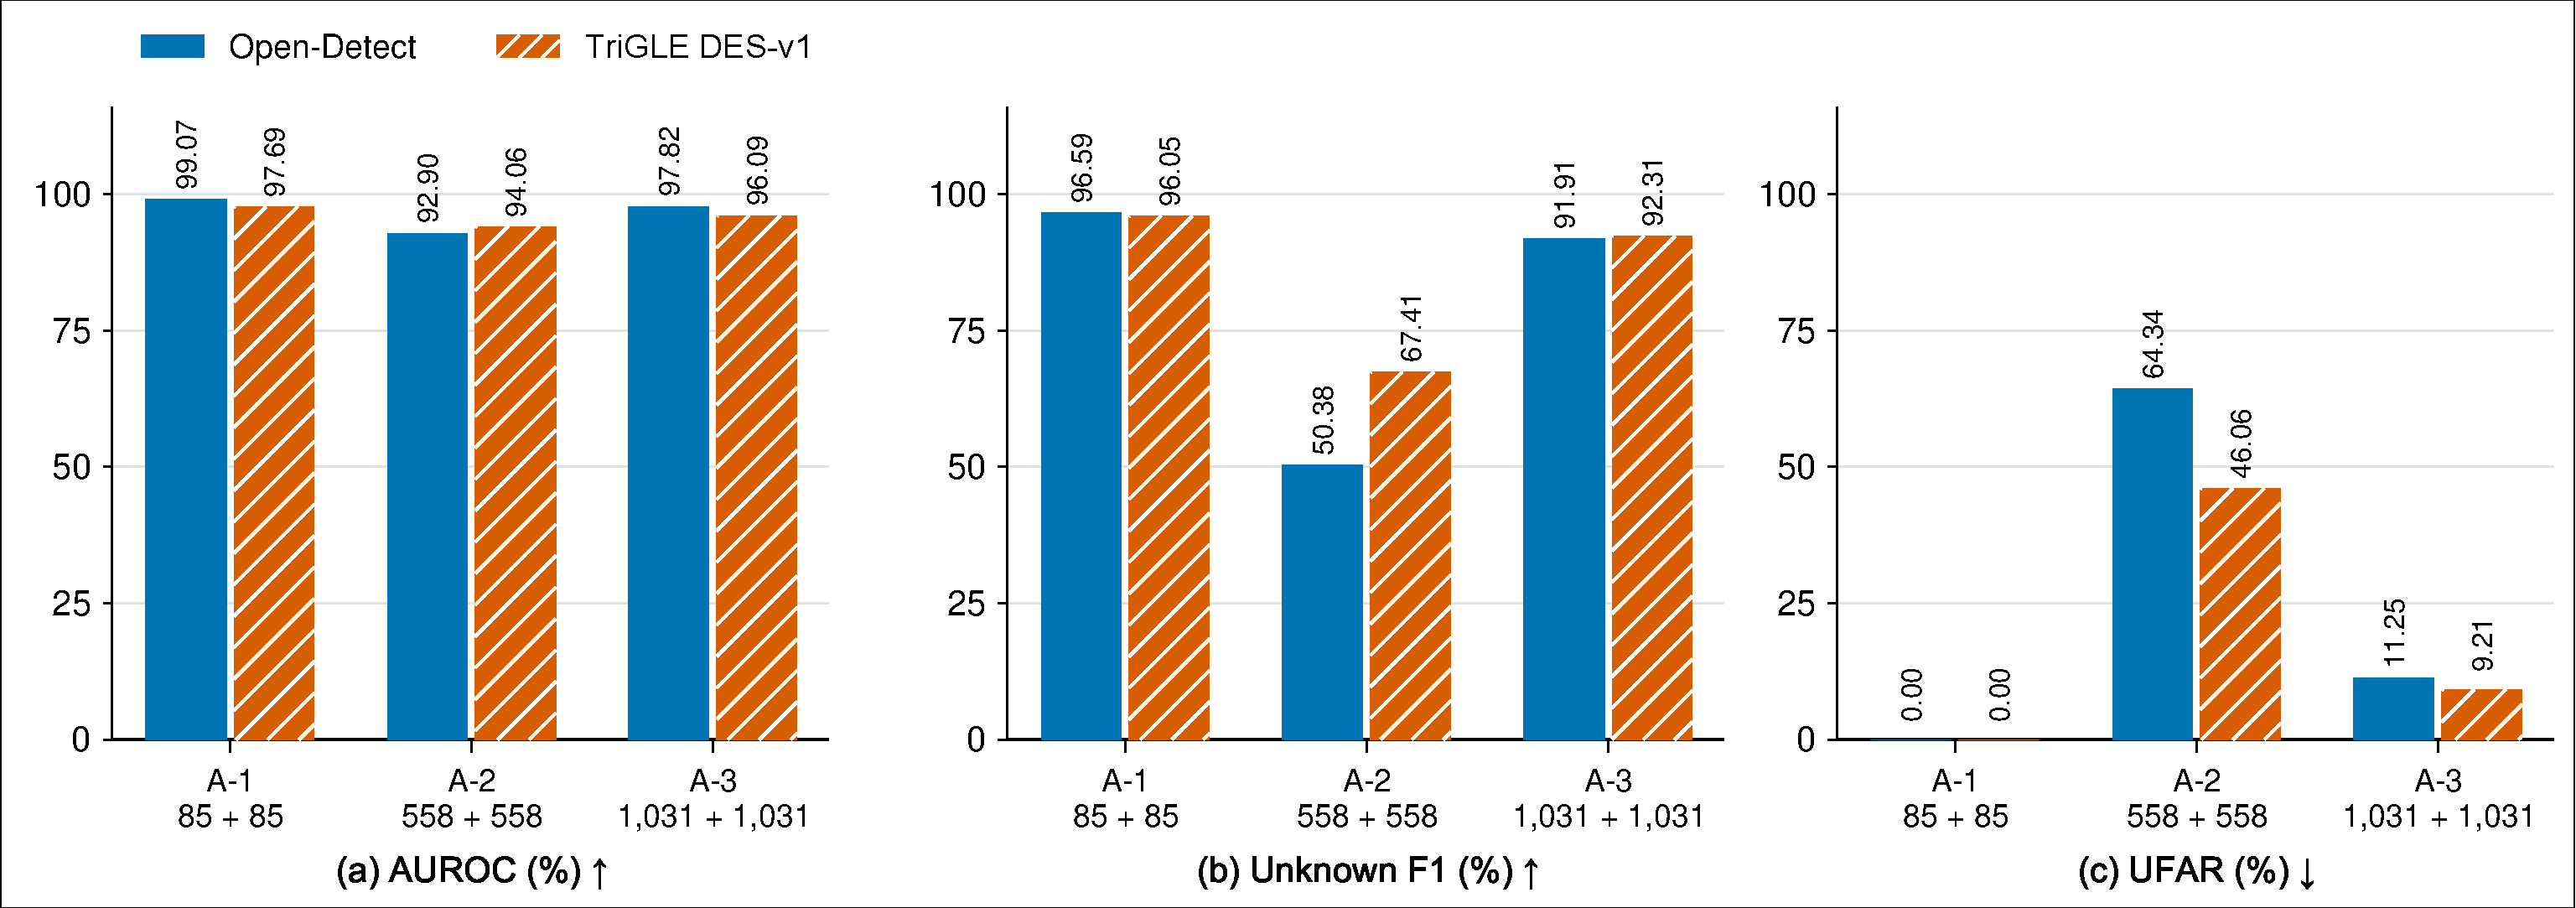
\includegraphics[width=0.96\textwidth,trim=3bp 3bp 3bp 3bp,clip,keepaspectratio]{images/suggestion3_fig4_1.pdf}
\begingroup
\renewcommand{\thefigure}{4-1}
\caption{Unknown-class detection performance under three USTC class-holdout configurations. (a) AUROC; (b) unknown-class F1; (c) UFAR.}
\label{fig:source-4-1}
\endgroup
\end{figure*}

\begin{figure*}[!t]
\centering
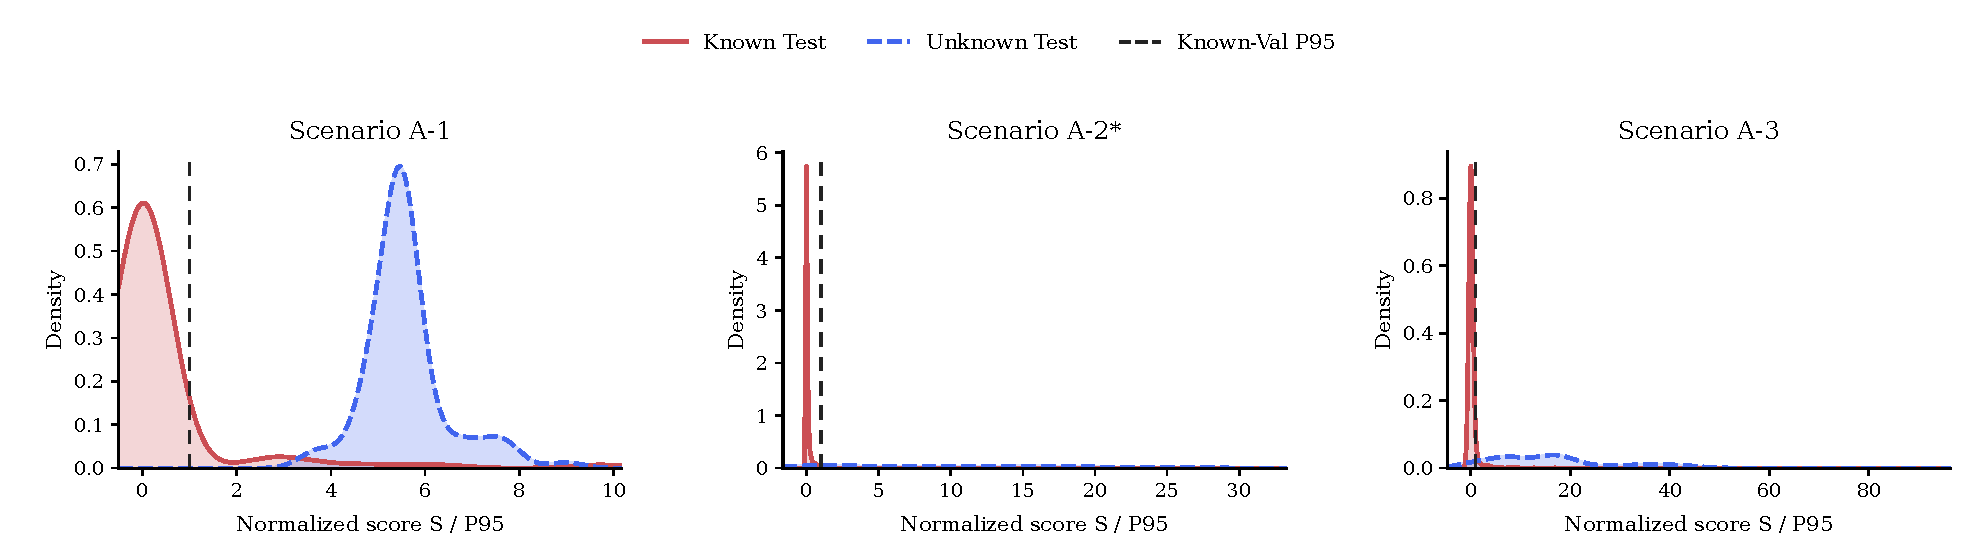
\includegraphics[width=0.98\textwidth,keepaspectratio]{images/ustc_score_distributions_normalized.pdf}
\begingroup
\renewcommand{\thefigure}{4-2}
\caption{Known and unknown score distributions in the USTC A-1, A-2, and A-3 settings.}
\label{fig:source-4-2}
\endgroup
\end{figure*}

\textbf{Class-level responses to unknown attacks.} Table~4-8 reports MSP and DES-v1 AUROC and DES-v1 AUPRC and UFAR for ten unknown CIC attacks. This comparison contrasts classification confidence with empirical support scores across attack scenarios.


\begin{table}[H]
\centering
\begingroup
\renewcommand{\thetable}{4-8}
\caption{Recognition results for ten unknown CIC attacks (\%, original test-pool proportions, P95)}\label{tab:source-8-cic}
\fontsize{7}{8.5}\selectfont
\setlength{\tabcolsep}{0pt}
\begin{tabular}{@{}>{\raggedright\arraybackslash}p{0.30\columnwidth}*{5}{>{\centering\arraybackslash}p{0.14\columnwidth}}@{}}
\hline
Unknown attack & \shortstack{Unknown\\flows} & \shortstack{MSP\\AUROC} & \shortstack{DES-v1\\AUROC} & \shortstack{DES-v1\\AUPRC} & \shortstack{DES-v1\\UFAR $\downarrow$} \\
\hline
DoS slowloris & 5,709 & 81.47 & \textbf{99.31} & 99.67 & 0.04 \\
DoS GoldenEye & 7,441 & 33.17 & \textbf{97.00} & 97.72 & 0.24 \\
DoS Hulk & 155,168 & 9.38 & \textbf{97.38} & 99.88 & 0.11 \\
FTP-Patator & 3,985 & 98.75 & \textbf{99.83} & 99.86 & 0.00 \\
SSH-Patator & 2,987 & 86.97 & \textbf{99.13} & 98.93 & 0.00 \\
Web Attack -- Brute Force & 1,364 & 91.61 & \textbf{99.57} & 99.14 & 0.00 \\
Web Attack -- XSS & 629 & 97.80 & \textbf{99.75} & 98.84 & 0.00 \\
DoS Slowhttptest & 5,096 & 85.97 & \textbf{99.34} & 99.63 & 0.14 \\
DDoS & 76,613 & 5.82 & \textbf{94.90} & 99.45 & 16.61 \\
Bot & 1,228 & 62.91 & \textbf{94.64} & 87.58 & 50.90 \\
\hline
\end{tabular}
\endgroup
\end{table}


DES-v1 achieves UFAR no greater than 0.24\% for eight of the ten unknown attacks, indicating effective rejection overall. Known FRR is 7.13\% for every attack category. For Hulk, MSP achieves only 9.38\% AUROC, whereas DES-v1 reaches 97.38\%, indicating that empirical support distance can compensate for classification-confidence failures on some unknown attacks. Bot and DDoS remain challenging, with UFAR values of 50.90\% and 16.61\%, respectively. This variation indicates that feature overlap between attack types and known classes affects rejection performance.

DDoS achieves 99.45\% AUPRC, but unknown samples account for 97.12\% of its original test pool and UFAR remains 16.61\%. Thus, under class imbalance, high AUPRC does not imply a low false acceptance rate at a fixed threshold. Rejection performance therefore requires joint assessment using ranking and threshold-dependent metrics. Together with VNAT and USTC, these results show effective overall unknown detection and recognition for most classes, while leaving room for improvement on unknown attacks whose feature distributions overlap those of known classes. We will address these difficult unknown classes in future work.

\subsection{Rejection Mechanism and Component Ablations}
\subsubsection{Roles of Global and Local Empirical Support}
To separate full-system gains from the contribution of the rejection rule, we fix the encoders, fused features $h(x)$, and classification outputs $\ell(x)$ across the four VNAT folds and change only the unknown-detection score. MSP and Energy use classification outputs. DES-v0 uses the squared distance to the nearest empirical centroid. DES-v1 incorporates the mean Euclidean distance to the 10 nearest neighbors within the nearest-centroid class. Each score independently calibrates its threshold on the known-class validation set. Table~4-9 presents the results.


\begin{table}[H]
\centering
\begingroup
\renewcommand{\thetable}{4-9}
\caption{Rejection scores on identical frozen representations (\%, equal-weight mean over four folds, original test-pool proportions, P95)}\label{tab:source-8}
\fontsize{8}{9.5}\selectfont
\setlength{\tabcolsep}{1pt}
\begin{tabular*}{\columnwidth}{@{\extracolsep{\fill}}lccccc@{}}
\hline
Rejection score & AUROC & AUPRC & Unknown F1 & UFAR & Known FRR \\
\hline
MSP & 91.83 & 96.66 & 90.55 & 14.63 & 4.93 \\
Energy & 91.73 & 96.58 & 89.96 & 15.40 & 4.87 \\
DES-v0 & 97.43 & 98.79 & 96.10 & 5.59 & 4.87 \\
\textbf{DES-v1} & \textbf{99.22} & \textbf{99.50} & \textbf{98.40} & \textbf{1.09} & \textbf{4.45} \\
\hline
\end{tabular*}
\par\smallskip\parbox{\columnwidth}{\fontsize{7}{8}\selectfont Note: DES-v0 uses empirical centroids only; DES-v1 combines global and local support. Higher AUROC, AUPRC, and Unknown F1 are better; lower UFAR and Known FRR are better.}
\endgroup
\end{table}


Local nearest-neighbor information further improves unknown detection on fixed representations. Compared with DES-v0, DES-v1 increases mean AUROC from 97.43\% to 99.22\%, reduces UFAR from 5.59\% to 1.09\%, and reduces Known FRR from 4.87\% to 4.45\%. For Remote Access, AUROC rises from 94.47\% to 98.76\%; for Communication, it rises from 98.24\% to 99.54\%. This comparison directly supports the combination of global and local empirical support in Section~III: neighborhoods of actual samples provide rejection information beyond class means. Fig.~4-4 visualizes these per-service differences.

The File Transfer fold further illustrates the trade-off between the two error rates. DES-v1 reduces Known FRR from 5.03\% to 4.61\%, while UFAR increases from 0.36\% to 0.56\%. Local support therefore primarily improves ranking across the four folds and average acceptance behavior. A specific operating point still requires joint assessment of false rejection of known services and false acceptance of unknown traffic.

\begin{figure*}[!t]
\centering
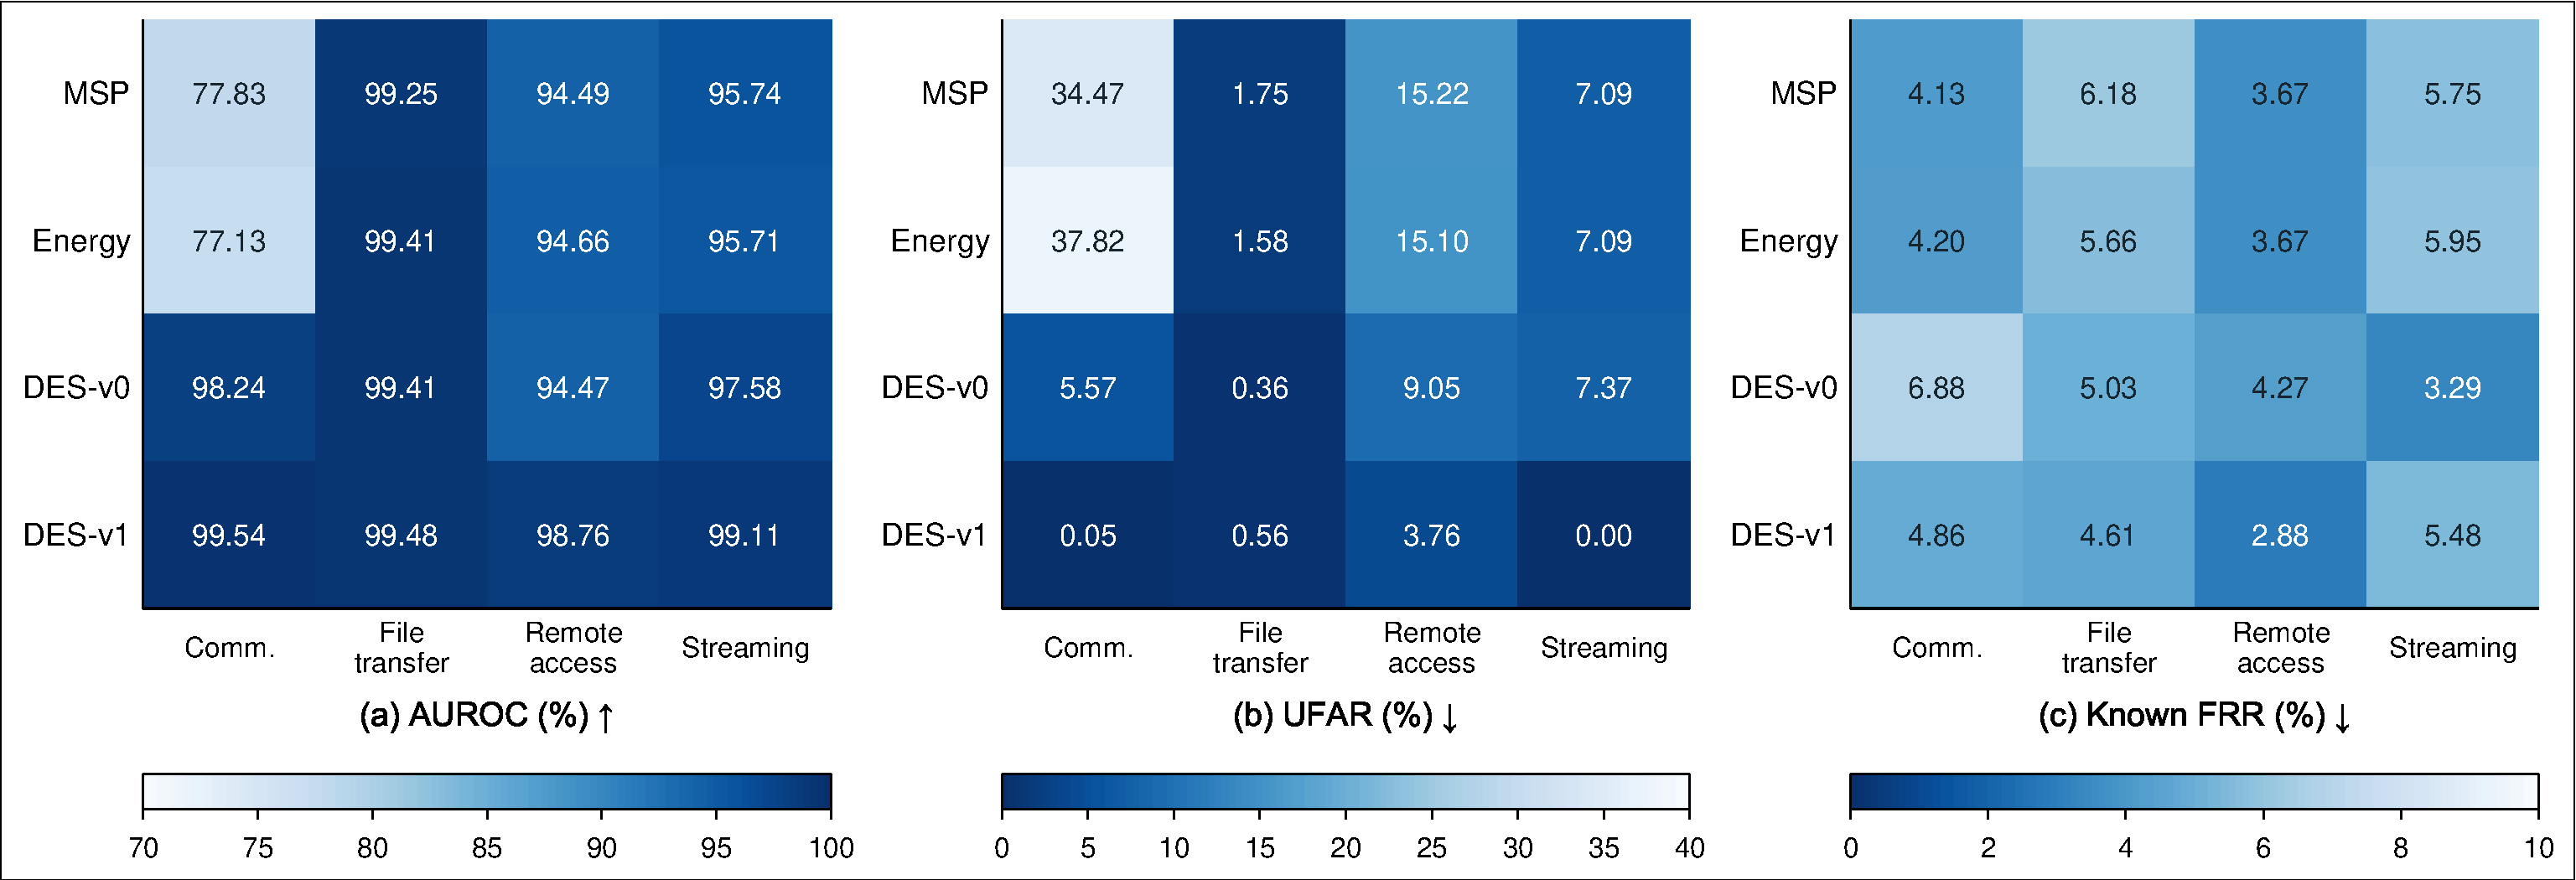
\includegraphics[width=0.88\textwidth,trim=4bp 4bp 4bp 4bp,clip,keepaspectratio]{images/Fig4_4_Reference.pdf}
\begingroup
\renewcommand{\thefigure}{4-4}
\caption{Ablation of rejection scores on identical TriGLE representations. Columns denote the four unknown services, and rows denote the four scores. The figure reports AUROC, UFAR, and Known FRR in sequence; all cells are percentages.}
\label{fig:source-4-3}
\endgroup
\end{figure*}

\subsubsection{View Contributions}
We ablate the FIG, YaTC, and TrafficFormer branches individually under the same four-fold VNAT configuration to assess each branch's contribution to the final representation. The encoders, Gaussian adapters, and normalization parameters remain frozen. All configurations retain the same fusion-head architecture and training settings for comparability. Table~4-10 reports closed-set classification and unknown-detection performance.


\begin{table}[H]
\centering
\begingroup
\renewcommand{\thetable}{4-10}
\caption{VNAT view ablations under the same configuration (\%, equal-weight mean over four folds, DES-v1, original test-pool proportions, P95)}\label{tab:source-9}
\fontsize{6.5}{8}\selectfont
\setlength{\tabcolsep}{1pt}
\begin{tabular}{@{}lcccccc@{}}
\hline
Configuration & Known Macro-F1 & AUROC & AUPRC & Unknown F1 & UFAR & Known FRR \\
\hline
TriGLE (full) & 99.87 & 99.22 & 99.50 & 98.40 & 1.09 & 4.45 \\
Without FIG & 97.08 & 97.45 & 97.37 & 97.24 & 1.41 & 3.49 \\
Without YaTC & 96.56 & 95.92 & 96.75 & 89.83 & 14.80 & 4.91 \\
Without TrafficFormer & 95.21 & 96.35 & 94.81 & 94.14 & 8.53 & 4.81 \\
\hline
\end{tabular}
\par\smallskip\parbox{\columnwidth}{\fontsize{7}{8}\selectfont Note: Higher Known Macro-F1, AUROC, AUPRC, and Unknown F1 are better; lower UFAR and Known FRR are better.}
\endgroup
\end{table}


Removing any branch degrades some key detection metrics in Table~4-10. Removing YaTC decreases unknown-class F1 from 98.40\% to 89.83\% and increases UFAR from 1.09\% to 14.80\%, indicating the importance of multilevel byte representations for separating unknown traffic from known classes. Removing TrafficFormer decreases AUPRC from 99.50\% to 94.81\% and unknown-class F1 to 94.14\%, indicating that contextual information in byte sequences complements known-class discrimination and unknown detection. Removing FIG decreases AUROC and AUPRC to 97.45\% and 97.37\%, respectively, decreases unknown-class F1 to 97.24\%, and increases UFAR to 1.41\%. These results indicate that the flow interaction graph provides structural information for traffic discrimination and unknown detection by modeling relationships between packets. Overall, the three views provide complementary information that jointly improves known-class recognition and unknown-class rejection.

\subsection{Sensitivity to the Rejection Threshold and Test Distribution}

\subsubsection{Effect of the Rejection Threshold}
The preceding results use the fixed P95 operating point. We retain the VNAT network, training support bank, and score, and additionally use P90 and P99 of the known-class validation scores to examine false acceptance and false rejection. Table~4-11 uses the existing four-fold results, with P95 remaining the primary operating point.


\begin{table}[H]
\centering
\begingroup
\renewcommand{\thetable}{4-11}
\caption{Sensitivity to validation-quantile thresholds on VNAT (\%, DES-v1, equal-weight mean over four folds, original test-pool proportions)}\label{tab:source-10}
\fontsize{7}{8.5}\selectfont
\setlength{\tabcolsep}{2pt}
\begin{tabular}{@{}cccc@{}}
\hline
Validation quantile & Unknown F1 $\uparrow$ & UFAR $\downarrow$ & Known FRR $\downarrow$ \\
\hline
P90 & 97.26 & 0.91 & 10.02 \\
P95 & 98.40 & 1.09 & 4.45 \\
P99 & 85.94 & 20.98 & 1.23 \\
\hline
\end{tabular}
\endgroup
\end{table}


The validation quantile directly controls the trade-off between acceptance of known samples and missed detection of unknown samples. P90 reduces mean UFAR to 0.91\% but increases Known FRR to 10.02\%. P99 reduces Known FRR to 1.23\% but increases UFAR to 20.98\%. A more permissive threshold increases known acceptance and may also increase missed unknown detections. All three operating points share the same score, so AUROC and AUPRC remain unchanged. Fixed-threshold error rates thus complement ranking metrics by characterizing acceptance behavior.

\subsubsection{Unknown Proportion and Class Composition}
Threshold sensitivity examines acceptance criteria under a fixed distribution, whereas mixed testing examines sample composition. From the frozen score pools for the ten CIC attacks, we draw 2,000 flows per trial and repeat the experiment using 20 deterministic seeds. With equal known and unknown proportions and equal representation of the ten unknown classes, DES-v1 achieves mean AUROC of 98.10\%, unknown-class F1 of 93.12\%, UFAR of 6.71\%, and Known FRR of 7.07\%. The model and P95 threshold remain frozen throughout.

Fig.~4-5 shows AUROC, AUPRC, UFAR, and Known FRR at five proportions of unknown traffic.

\begin{figure}[H]
\centering
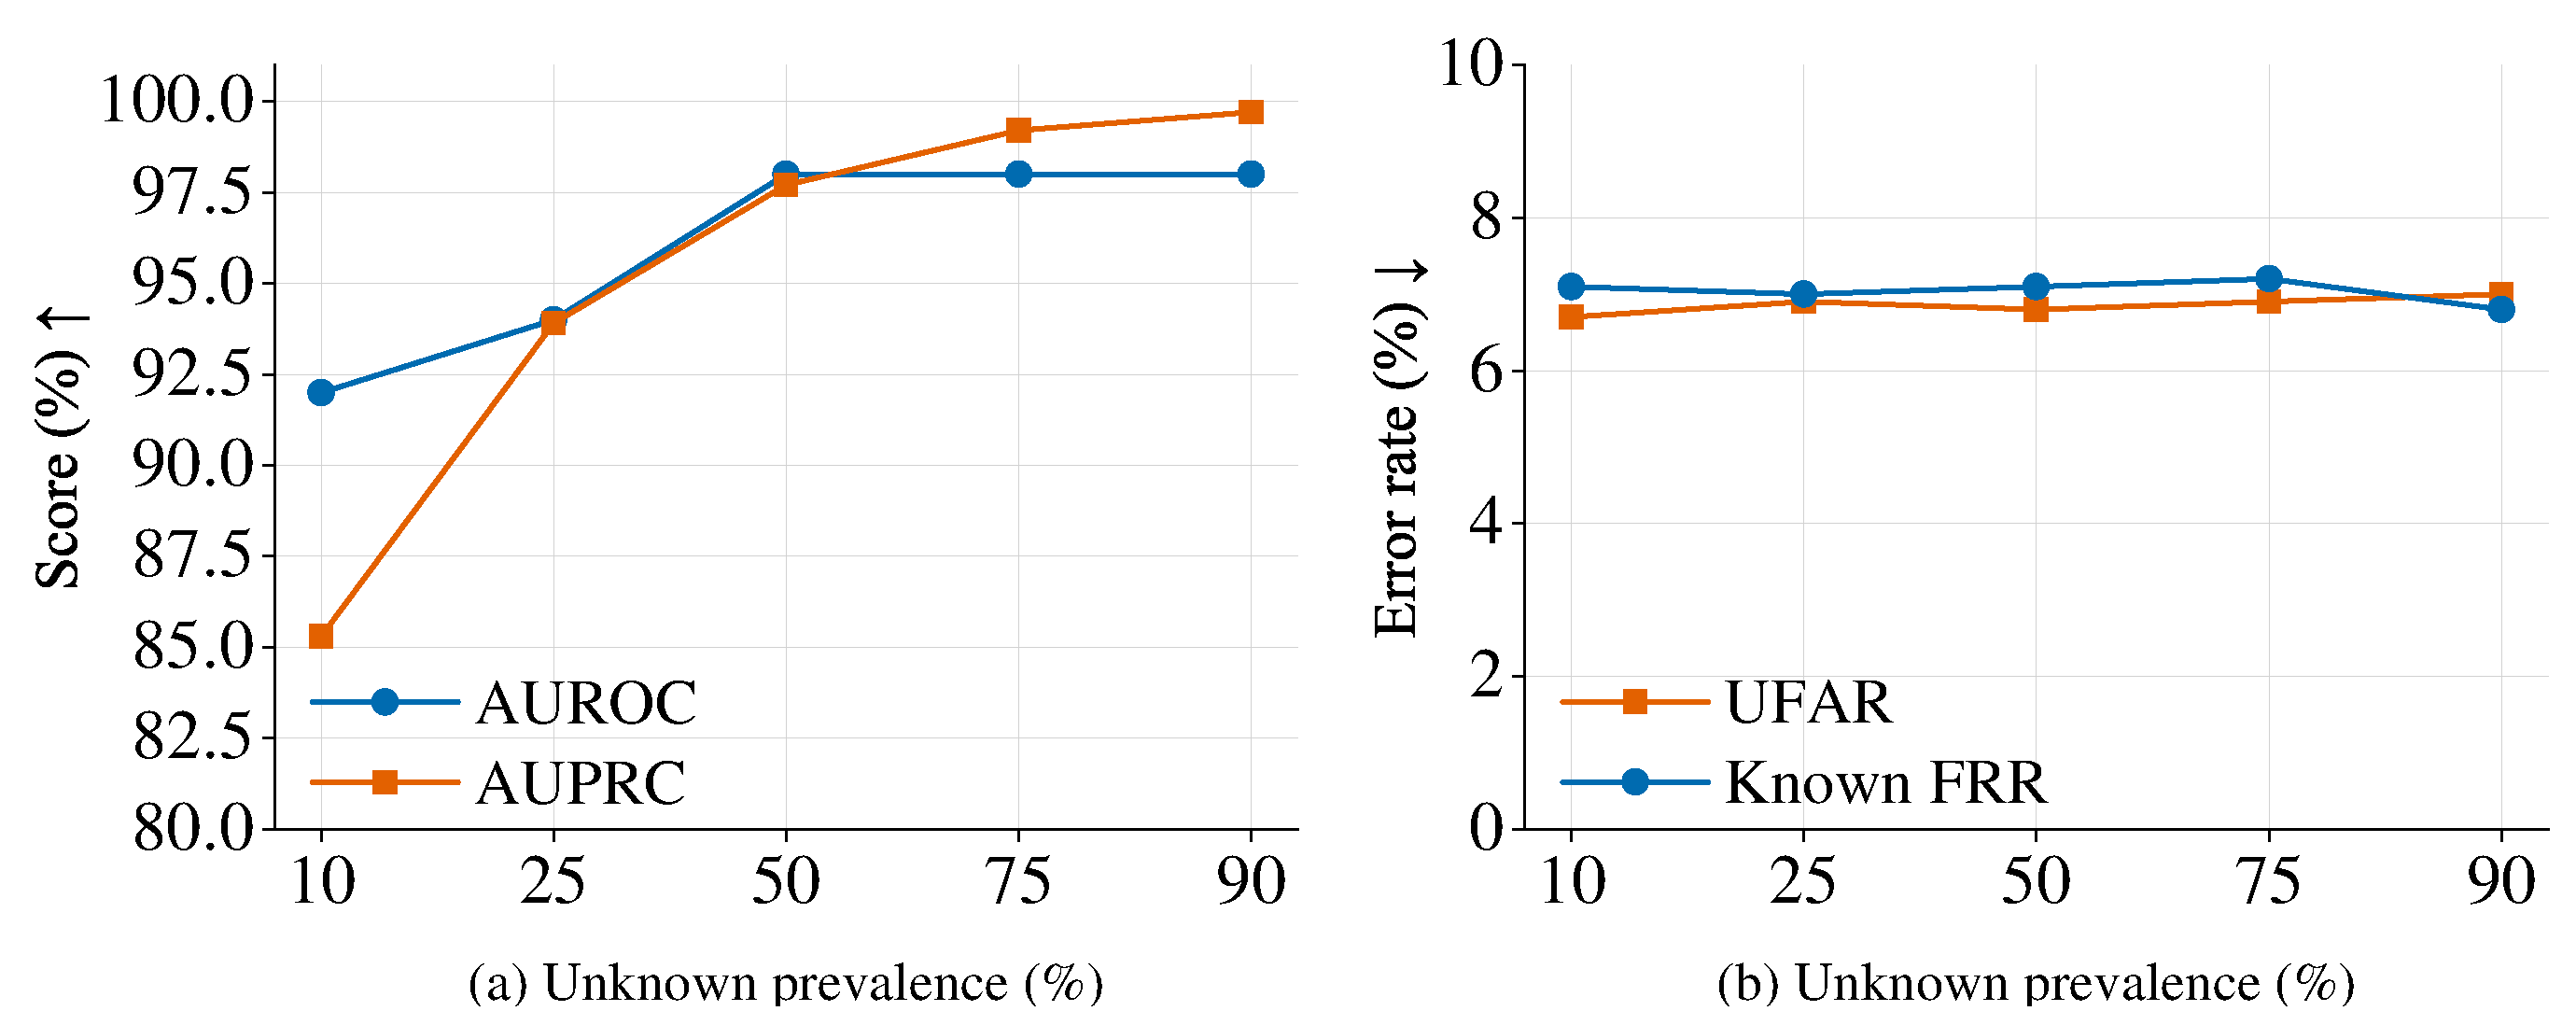
\includegraphics[width=\columnwidth,keepaspectratio]{images/suggestion2_fig4_5.pdf}
\begingroup
\renewcommand{\thefigure}{4-5}
\caption{Prevalence sensitivity across five equally spaced settings. (a) AUROC and AUPRC. (b) UFAR and Known FRR.}
\label{fig:source-4-4}
\endgroup
\end{figure}

Ranking performance and conditional error rates remain relatively stable as the proportion of unknown samples changes. With the ten unknown classes balanced internally and the known-to-unknown ratio varying from 9:1 to 1:9, Fig.~4-5 shows AUROC ranging from approximately 92.0\% to 98.0\% and UFAR from approximately 6.7\% to 7.0\%. AUPRC increases from approximately 85.3\% to 99.7\% as the unknown proportion rises. At a fixed 1:1 ratio, mixing only Bot and DDoS attack samples increases UFAR to 33.84\%. Changes in the composition of normal traffic and PortScan also affect Known FRR. Together with the per-attack results, these findings indicate that the detector is more sensitive to unknown-class composition than to the overall proportion of unknown samples.

\section{Conclusion}
The experiments show that TriGLE classifies known traffic and rejects many unknown services and attacks under the stated protocols.\par\smallskip
\textbf{Limitations:} We validate the proposed method on multiple public datasets and under different unknown-class holdout settings, but dataset provenance and traffic distributions constrain the experiments. The datasets differ in capture environments, application types, and traffic composition. Unknown-class feature distributions also strongly affect rejection performance. The model still falsely accepts some unknown traffic whose features resemble those of known classes.

\textbf{Future work:} We will expand dataset and experimental coverage through cross-dataset and cross-network-environment generalization tests to assess adaptation to different traffic distributions. To address feature overlap between unknown and known classes, we will investigate more effective local feature modeling and rejection strategies for difficult unknown classes. We will also examine the effects of packet padding, segmentation, and traffic perturbations on multiview representations and explore detection methods that depend less on raw bytes to improve robustness in complex network environments.

\endgroup

\begin{thebibliography}{18}
\bibitem{ch2-1} X. Lin et al., ``ET-BERT: A Contextualized Datagram Representation with Pre-training Transformers for Encrypted Traffic Classification,'' WWW, 2022, doi: \url{10.1145/3485447.3512217}.
\bibitem{ch2-2} G. Zhou et al., ``TrafficFormer: An Efficient Pre-trained Model for Traffic Data,'' IEEE S\&P, 2025, doi: \url{10.1109/SP61157.2025.00102}.
\bibitem{ch2-3} X. Y. Chen et al., ``MIETT: Multi-Instance Encrypted Traffic Transformer for Encrypted Traffic Classification,'' AAAI, 2025, doi: \url{10.1609/aaai.v39i15.33748}.
\bibitem{ch2-4} R. Zhao et al., ``Yet Another Traffic Classifier: A Masked Autoencoder Based Traffic Transformer with Multi-Level Flow Representation,'' AAAI, 2023, doi: \url{10.1609/aaai.v37i4.25674}.
\bibitem{ch2-5} M. Shen et al., ``Accurate Decentralized Application Identification via Encrypted Traffic Analysis Using Graph Neural Networks,'' IEEE TIFS, 2021, doi: \url{10.1109/TIFS.2021.3050608}.
\bibitem{ch2-6} H. Zhang et al., ``TFE-GNN: A Temporal Fusion Encoder Using Graph Neural Networks for Fine-grained Encrypted Traffic Classification,'' WWW, 2023, doi: \url{10.1145/3543507.3583227}.
\bibitem{ch2-7} H. Zhang et al., ``Revolutionizing Encrypted Traffic Classification with MH-Net: A Multi-View Heterogeneous Graph Model,'' AAAI, 2025, doi: \url{10.1609/aaai.v39i1.32091}.
\bibitem{ch2-8} X. Qiu et al., ``Dual-Channel Interactive Graph Transformer for Traffic Classification with Message-Aware Flow Representation,'' AAAI, 2025, doi: \url{10.1609/aaai.v39i1.32050}.
\bibitem{ch2-9} J. Zhang et al., ``Autonomous Unknown-Application Filtering and Labeling for DL-based Traffic Classifier Update,'' INFOCOM, 2020, doi: \url{10.1109/INFOCOM41043.2020.9155292}.
\bibitem{ch2-10} Q. Yang et al., ``End-to-End Open-Set Semi-Supervised Learning for Fine-Grained Encrypted Traffic Classification,'' IEEE TIFS, 2026, doi: \url{10.1109/TIFS.2026.3653575}.
\bibitem{ch2-11} Z. Zhao et al., ``FOSS: Towards Fine-Grained Unknown Class Detection Against the Open-Set Attack Spectrum With Variable Legitimate Traffic,'' IEEE/ACM ToN, 2024, doi: \url{10.1109/TNET.2024.3413789}.
\bibitem{ch2-12} Y. Zhong et al., ``RFG-HELAD: A Robust Fine-Grained Network Traffic Anomaly Detection Model Based on Heterogeneous Ensemble Learning,'' IEEE TIFS, 2024, doi: \url{10.1109/TIFS.2024.3402439}.
\bibitem{ch2-13} Z. Zhao et al., ``Trident: A Universal Framework for Fine-Grained and Class-Incremental Unknown Traffic Detection,'' WWW, 2024, doi: \url{10.1145/3589334.3645407}.
\bibitem{ch2-14} J. Yang et al., ``Conditional Variational Auto-Encoder and Extreme Value Theory Aided Two-Stage Learning Approach for Intelligent Fine-Grained Known/Unknown Intrusion Detection,'' IEEE TIFS, 2021, doi: \url{10.1109/TIFS.2021.3083422}.
\bibitem{ch2-15} Q. Meng et al., ``Detection of Unknown Attacks Through Encrypted Traffic: A Gaussian Prototype-Aided Variational Autoencoder Framework,'' IEEE TIFS, 2025, doi: \url{10.1109/TIFS.2025.3612141}.
\bibitem{ch2-16} X. Wang, Y. Wang, Y. Lai, Z. Hao, and A. X. Liu, ``Reliable Open-Set Network Traffic Classification,'' IEEE Trans. Inf. Forensics Secur., vol. 20, pp. 2313--2328, 2025, doi: \url{10.1109/TIFS.2025.3544067}.
\bibitem{ch2-17} D. Hendrycks and K. Gimpel, ``A Baseline for Detecting Misclassified and Out-of-Distribution Examples in Neural Networks,'' ICLR, 2017.
\bibitem{ch2-18} W. Liu, X. Wang, J. Owens, and Y. Li, ``Energy-based Out-of-distribution Detection,'' NeurIPS, vol. 33, 2020.
\end{thebibliography}
\end{document}
